\chapter{Verifica e validazione}
\label{cap:verifica-validazione}

\intro{In questo capitolo vengono riportati tutti i dati e le prove effettuate sul RALM per ogni modifica aggiunta}

\section{Test}
Come fonte di informazioni per il RALM sono state scelte cinque pagine di Wikipedia e sono state convertite nei formati desiderati (HTML, Pdf, Docx).
La pagine scelte sono composte di testo e altri elementi semantici, tra cui le tabelle che hanno la struttura della tabella \ref{tab:esempio-cibo} spiegata nel paragrafo \nameref{subsubsec-lin-tab}

I test sono stati effettuati tramite una valutazione umana secondo i seguenti criteri:
\begin{itemize}
    \item La risposta deve essere ben strutturata, scritta in maniera corretta e comprensibile;
    \item La risposta deve essere corretta e completa.
\end{itemize}

Sulla base di ciò a ogni risposta viene assegnato un valore tra 0 (risposta non corretta/strutturata male) e 1 (risposta corretta e strutturata correttamente)

\subsection{Domande}
Sono stati creati due set da 10 domande l'uno, le domande sono state create in maniera tale da poter interrogare il modello sui dati presenti nelle tabelle dei vari documenti:
\begin{itemize}
    \item Set di domande semplici: domande che interrogano il RALM su singole celle delle tabelle o celle che hanno la stessa intestazione;
    \item Set di domande complesse: domande che interrogano il RALM su diverse celle e che chiedono di fare diverse operazioni tra i dati presenti (es: somma, media).
\end{itemize}

\subsubsection{Set di domande semplici}
\begin{table}[H]
    \centering
    \begin{tabular}{|p{0.5cm} |p{2.5cm} |p{4cm}| p{4.5cm}|}
        \hline
        \textbf{N}. & \textbf{Nome pagina} & \textbf{Domanda} & \textbf{Risposta corretta} \\
        \hline
        1 & Italia & Quali sono le 3 città italiane con più abitanti? & Roma, Milano, Napoli \\
        \hline
        2 & Italia & Nel settore terziario italiano, qual è il settore che presenta più imprese? & Il commercio \\
        \hline
        3 & Avanti un altro! & In quali paesi è stato esportato Avanti un altro? & Spagna, Albania, Ungheria, Vietnam, Brasile, Bulgaria, Cile, Paraguay, Canada, Turchia, Polonia, Romania \\
        \hline
        4 & Avanti un altro! & In che canale è stato trasmesso Avanti un altro? & Canale 5\\
        \hline
        5 & SPAR & In che anno è arrivato SPAR in italia? & 1959 \\
        \hline
        6 & SPAR & Quanto volume d'affari ha SPAR in Belgio & 626.307 \\
        \hline
        7 & The Space Cinema & Quante sale ha il The Space Cinema di Padova? & 14 \\
        \hline
        8 & The Space Cinema & Quanti posti a sedere ha il The Space Cinema di Parma centro & 1402 \\
        \hline
        9 & Sonic(serie) & In che anno è uscito il videogioco "Sonic Battle"? & 2003 \\
        \hline
        10 & Sonic(serie) & Dov'è apparso Tails per la prima volta? & Sonic the hedghog 2 \\
        \hline
    \end{tabular}
    \caption{Set di domande semplici poste al RALM}
\end{table}

\subsubsection{Set di domande complesse}
\begin{table}[H]
    \centering
    \begin{tabular}{|p{0.5cm} |p{2.5cm} |p{4cm}| p{4.5cm}|}
        \hline
        \textbf{N}. & \textbf{Nome pagina} & \textbf{Domanda} & \textbf{Risposta corretta} \\
        \hline
        1 & Italia & Quali città hanno più di 500000 abitanti in italia? & Roma, Milano, Napoli, Torino, Palermo e Genova \\
        \hline
        2 & Italia & Quali sono le città italiane che hanno più 300000 abitanti ma meno di 387841? & Firenze, Bari, Catania \\
        \hline
        3 & Avanti un altro! & Mediamente quanti telespettatori ci sono stati per ogni edizione di avanti un altro? & circa 3700000 \\
        \hline
        4 & Avanti un altro! & Quante puntate ci sono state di avanti un altro in tutto? & Circa 1400 \\
        \hline
        5 & SPAR & In quali paesi è arrivato SPAR dal 2000 in poi? & Russia, Mauritius, Cipro, Ucraina, Cina, Croazia \\
        \hline
        6 & SPAR & In quali paesi le strutture SPAR hanno meno di 10000 metri quadrati di superficie? & Croazia, Mauritious, Zambia,  India, Albania \\
        \hline
        7 & The Space Cinema & Quali sono i the space situati in provincia di Torino? & Beinsasco, Torino - Parco Dora \\
        \hline
        8 & The Space Cinema & Quali sono i the space con più di 13 sale? & Limena, Roma Paroc de' Medici,  Vimercate \\
        \hline
        9 & Sonic(serie) & Chi è eggman e quando ha fatto la sua prima apparizione? & Eggman è un uomo esperto di ingegneria robotica che vuole conquistare il mondo di Sonic, antagonista principale della serie. Ha fatto la sua prima apparizione in "Sonic the hedghog". \\
        \hline
        10 & Sonic(serie) & Elenca tutti i giochi mobile di Sonic dal 2015 in poi & Sonic runners, sonic dash 2: sonic boom, sonic runners adventure, sonic forces speed battle, sonic speed simulaor \\
        \hline
    \end{tabular}
    \caption{Set di domande complesse poste al RALM}
\end{table}

Nei seguenti paragrafi vengono riportate le risposte del RALM a ogni aggiornamento significativo del codice per denotare l'effettivo miglioramento della qualità delle risposte:

\begin{enumerate}
    \item Prima versione: estrazione del contenuto semplice (senza linearizzazione delle tabelle, senza correzione del chunking e pulizia del testo);
    \item Seconda verione: estrazione del contenuto con la linearizzazione delle tabelle;
    \item Terza versione: estrazione del contenuto con la linearizzazione delle tabelle e la correzione del chunking e pulizia del testo;

\end{enumerate}


\subsection{Test sui file HTML}

\subsubsection{Prima versione - Risposte al set di domande semplici}

\begin{table}[H]
    \centering
    \begin{tabular}{|p{0.5cm} |p{6cm} |p{2cm}|}
        \hline
        \textbf{N}. & \textbf{Risposta fornita dal RALM} & \textbf{Valutazione} \\
        \hline
        1 & Roma, Milano e Napoli sono le tre città italiane con più abitanti. & 1 \\
        \hline
        2 & Il settore che presenta più imprese nel terziario italiano è il settore dei servizi. & 0 \\
        \hline
        3 & Avanti un altro! è stato esportato in Spagna, Albania, Ungheria, Vietnam, Brasile, Paraguay, Cile, Bulgaria, Canada, Turchia, Polonia e Romania. & 1 \\
        \hline
        4 & Avanti un altro è stato trasmesso sul canale 5. & 1 \\
        \hline
        5 & SPAR è arrivato in Italia nel 1959. & 1 \\
        \hline
        6 &  SPAR in Belgio & 0 \\
        \hline
        7 & Il the space di Padova ha 14 sale & 1 \\
        \hline
        8 & Il The Space di Parma Centro ha 7 sale e 1402 posti a sedere & 1 \\
        \hline
        9 & Il videogioco Sonic Battle è stato pubblicato da Sega nel 2003. & 1 \\
        \hline
        10 & Tails è un compagno di Sonic che appare per la prima volta in Sonic the Hedgehog 2 nel 1992. & 1 \\
        \hline
    \end{tabular}
    \caption{Risposte al set di domande semplici date dalla prima versione del RALM (File HTML)}
\end{table}

\textbf{Correttezza:} 8/10

\subsubsection{Prima versione - Risposte al set di domande complesse}

\begin{table}[H]
    \centering
    \begin{tabular}{|p{0.5cm} |p{6cm} |p{2cm}|}
        \hline
        \textbf{N}. & \textbf{Risposta fornita dal RALM} & \textbf{Valutazione} \\
        \hline
        1 & Palermo, Cagliari, Trento, Venezia, Trieste, Bologna, Firenze, Perugia, Ancona, Roma, Napoli, Bari, Potenza, Catanzaro, Matera, Belluno & 0 \\
        \hline
        2 & Napoli, Palermo, Genova, Bologna, Firenze e Bari. & 0 \\
        \hline
        3 & In media si contano 3.995.000 spettatori per edizione. & 0.8 \\
        \hline
        4 & 17 edizioni, con una puntata speciale & 0 \\
        \hline
        5 & SPAR è arrivata in Belgio, Danimarca, Francia, Germania, Irlanda, Italia, Lituania, Paesi Bassi, Polonia, Regno Unito, Russia, Sudafrica, Spagna, Svizzera, Ungheria, Zimbabwe. & 0 \\
        \hline
        6 & SPAR è presente in Croazia, Slovenia, Austria, Germania, Regno Unito, Italia, Sudafrica, Norvegia, Giappone, Cina e Croazia. & 0 \\
        \hline
        7 & The Space Cinema è una catena di cinema presente in provincia di Torino. Ha 8 sale e 1295 posti a sedere. & 0 \\
        \hline
        8 & The Space Cinema è una delle catene di cinema più grandi in Italia, con 34 diverse strutture e 347 sale.  & 0 \\
        \hline
        9 & Eggman è un personaggio che è appena comparso nella serie Sonic. È uno scienziato malvagio che cerca di conquistare il mondo. & 0 \\
        \hline
        10 & Sonic mobile games from 2015 onwards: Sonic Jump (2015), Sonic Dash (2013), Sonic Jump Fever (2014), Sonic Runners (2015), Sonic Dash 2: Sonic Boom (2015), Sonic Runners Adventure (2017), Sonic Forces: Speed Battle (2017), Sonic Speed Simulator (2022) & 0 \\
        \hline
    \end{tabular}
    \caption{Risposte al set di domande complesse date dalla prima versione del RALM (File HTML)}
\end{table}

\textbf{Correttezza:} 0.8/10

\subsubsection{Seconda versione - Risposte al set di domande semplici}

\begin{table}[H]
    \centering
    \begin{tabular}{|p{0.5cm} |p{6cm} |p{2cm}|}
        \hline
        \textbf{N}. & \textbf{Risposta fornita dal RALM} & \textbf{Valutazione} \\
        \hline
        1 & Roma, Milano e Napoli sono le prime tre città italiane per popolazione. & 1 \\
        \hline
        2 & Il commercio è il settore che presenta più imprese in Italia, seguito da turismo, trasporti e logistica, e altri servizi. & 1 \\
        \hline
        3 & Avanti un altro! è stato esportato in Spagna, Albania, Ungheria, Vietnam, Brasile, Paraguay, Cile, Bulgaria, Canada, Turchia, Polonia e Romania. & 1 \\
        \hline
        4 & Avanti un altro è stato trasmesso sul canale 5. & 1 \\
        \hline
        5 & SPAR è arrivato in Italia nel 1959. & 1 \\
        \hline
        6 & SPAR ha un volume d'affari di 626.307 migliaia di € in Belgio. & 1 \\
        \hline
        7 & Il the space di Padova ha 14 sale & 1 \\
        \hline
        8 & The Space Cinema di Parma Centro ha 1402 posti a sedere. & 1 \\
        \hline
        9 & Il videogioco Sonic Battle è uscito nel 2003. & 1 \\
        \hline
        10 & Tails ha fatto la sua prima apparizione in Sonic the Hedgehog 2 (8-bit) nel 1992. Da allora, è apparso in un totale di 56 giochi. & 1 \\
        \hline
    \end{tabular}
    \caption{Risposte al set di domande semplici date dalla seconda versione del RALM (File HTML)}
\end{table}

\textbf{Correttezza:} 10/10

\subsubsection{Seconda versione - Risposte al set di domande complesse}

\begin{table}[H]
    \centering
    \begin{tabular}{|p{0.5cm} |p{6cm} |p{2cm}|}
        \hline
        \textbf{N}. & \textbf{Risposta fornita dal RALM} & \textbf{Valutazione} \\
        \hline
        1 & Le città italiane con più di 500.000 abitanti sono Milano, Roma, Torino, Palermo, Napoli e Genova. & 1 \\
        \hline
        2 & Firenze, Bari, Catania & 1 \\
        \hline
        3 & Non è chiaro quanto sia l'edizione di Avanti un altro, ma si stima che ci siano stati 3 milioni di telespettatori per edizione. & 0 \\
        \hline
        4 & In totale, ci sono stati 1.143 episodi di "Avanti un altro!" trasmessi dal 2011 al 2020. & 0 \\
        \hline
        5 & I Paesi in cui è arrivato SPAR dal 2000 in poi sono Russia, Mauritius, Cipro, Ucraina, Cina e Croazia. & 1 \\
        \hline
        6 & I paesi in cui le strutture SPAR hanno meno di 10000 metri quadrati di superficie sono la Polonia, l'Australia, l'Ucraina, la Croazia e lo Zimbabwe. & 0 \\
        \hline
        7 & I nomi dei the space situati in provincia di Torino sono Montesilvano, Napoli, Nola, Parma Campus, Parma Centro e Pradamano. & 0 \\
        \hline
        8 & I cinema The Space con più di 13 sale sono: Rozzano, Salerno, Sestu, Silea. & 0 \\
        \hline
        9 & Eggman è un personaggio che appare nella serie Sonic. È un uomo esperto di ingegneria robotica che vuole conquistare il mondo di Sonic. Ha fatto la sua prima apparizione in Sonic the Hedgehog nel 1991.  & 1 \\
        \hline
        10 & I giochi mobile di Sonic dal 2015 in poi sono: Sonic runners (2015), Sonic Dash 2: Sonic Boom (2015), Sonic Runners Adventure (2017), Sonic Forces: Speed Battle (2017) e Sonic Speed Simulator (2022). & 1 \\
        \hline
    \end{tabular}
    \caption{Risposte al set di domande complesse date dalla seconda versione del RALM (File HTML)}
\end{table}

\textbf{Correttezza:} 5/10

\subsection{Test sui file Docx}

\subsubsection{Prima versione - Risposte al set di domande semplici}

\begin{table}[H]
    \centering
    \begin{tabular}{|p{0.5cm} |p{6cm} |p{2cm}|}
        \hline
        \textbf{N}. & \textbf{Risposta fornita dal RALM} & \textbf{Valutazione} \\
        \hline
        1 & Roma, Milano e Napoli. & 1 \\
        \hline
        2 & Il settore terziario, composto principalmente da commercio, trasporti e logistica, turismo e altri servizi, rappresenta la maggior parte delle imprese italiane. & 0 \\
        \hline
        3 & Il format è stato ideato da Paolo Bonolis e Stefano Santucci ed è stato esportato in: Spagna, Albania, Ungheria, Vietnam, Brasile, Paraguay, Cile, Bulgaria, Canada, Turchia, Polonia e Romania. & 1 \\
        \hline
        4 & Avanti un altro! è un game show italiano in onda su Canale 5. Il programma va in onda dallo studio 1 del Centro Titanus Elios di Roma. & 1 \\
        \hline
        5 & Il marchio SPAR è arrivato in Italia nel 1959. & 1 \\
        \hline
        6 & SPAR ha un volume d'affari di 29,7 miliardi di euro in Belgio. & 0 \\
        \hline
        7 & The Space Cinema di Padova ha 14 sale. & 1 \\
        \hline
        8 & Il The Space di Parma Centro ha 7 sale e una capienza massima di 1.402 posti a sedere. & 1 \\
        \hline
        9 & Il videogioco Sonic Battle è stato lanciato nel 2003. & 1 \\
        \hline
        10 & Tails è apparso per la prima volta in Sonic the Hedgehog 2 nel 1992. & 1 \\
        \hline
    \end{tabular}
    \caption{Risposte al set di domande semplici date dalla prima versione del RALM (File Docx)}
\end{table}

\textbf{Correttezza:} 8/10

\subsubsection{Prima versione - Risposte al set di domande complesse}

\begin{table}[H]
    \centering
    \begin{tabular}{|p{0.5cm} |p{6cm} |p{2cm}|}
        \hline
        \textbf{N}. & \textbf{Risposta fornita dal RALM} & \textbf{Valutazione} \\
        \hline
        1 & Roma, Milano, Napoli, Torino, Palermo, Genova, Bologna, Firenze, Bari, Catania & 0 \\
        \hline
        2 & Napoli, Palermo, Genova, Bologna, Firenze e Bari. & 0 \\
        \hline
        3 & Nelle prime quattro stagioni era presente in studio come responsabile della sicurezza il buttafuori Mediaset Girolamo Di Stolfo, noto come Big Jimmy, poi ricordato da Bonolis al termine della prima puntata della quinta edizione, in seguito alla sua morte avvenuta il 13 luglio 2015 per aneurisma cerebrale. & 0 \\
        \hline
        4 & Circa 1000. & 0 \\
        \hline
        5 & SPAR è presente in 32 paesi in tutto il mondo. & 0 \\
        \hline
        6 & I paesi in cui le strutture SPAR hanno meno di 10000 metri quadrati di superficie sono l'Albania, l'Austria, la Germania, il Regno Unito, l'Italia, la Sudafrica, il Giappone, la Spagna e l'Irlanda. & 0 \\
        \hline
        7 & There are 9 The Space Cinemas located in the province of Turin. & 0 \\
        \hline
        8 & The Space Cinema è una catena di multisale cinematografiche che opera in Italia. È la seconda catena di cinema più grande sul territorio italiano, superata solo dal circuito United Cinemas International. & 0 \\
        \hline
        9 & Il Dr. Robotnik alias Eggman è un uomo esperto di ingegneria robotica che vuole conquistare il mondo di Sonic, antagonista principale della serie. & 0.5 \\
        \hline
        10 & I giochi mobile di Sonic dal 2015 sono: Sonic Dash 2: Sonic Boom, Sonic Runners Adventure, Sonic Forces: Speed Battle, Sonic Speed Simulator. & 1 \\
        \hline
    \end{tabular}
    \caption{Risposte al set di domande complesse date dalla prima versione del RALM (File Docx)}
\end{table}

\textbf{Correttezza:} 1.5/10

\subsubsection{Seconda versione - Risposte al set di domande semplici}

\begin{table}[H]
    \centering
    \begin{tabular}{|p{0.5cm} |p{6cm} |p{2cm}|}
        \hline
        \textbf{N}. & \textbf{Risposta fornita dal RALM} & \textbf{Valutazione} \\
        \hline
        1 & Le 3 città italiane con più abitanti sono: Roma, Milano e Napoli. & 1 \\
        \hline
        2 & Il settore che presenta più imprese nel settore terziario italiano è il commercio. & 1 \\
        \hline
        3 & Il format Avanti un altro! è stato esportato in Spagna, Albania, Ungheria, Vietnam, Brasile, Paraguay, Cile, Bulgaria, Canada, Turchia, Polonia e Romania. & 1 \\
        \hline
        4 & Avanti un altro è stato trasmesso  nel preserale di Canale 5 & 1 \\
        \hline
        5 & 1959 & 1 \\
        \hline
        6 & 626.307 & 1 \\
        \hline
        7 & The Space Cinema ha 14 sale e 3178 posti a sedere. & 1 \\
        \hline
        8 & 1402 & 1 \\
        \hline
        9 & Il videogioco Sonic Battle è uscito nel 2003. & 1 \\
        \hline
        10 & Tails è apparso per la prima volta in Sonic the Hedgehog 2 nel 1992. & 1 \\
        \hline
    \end{tabular}
    \caption{Risposte al set di domande semplici date dalla seconda versione del RALM (File Docx)}
\end{table}

\textbf{Correttezza:} 10/10

\subsubsection{Seconda versione - Risposte al set di domande complesse}

\begin{table}[H]
    \centering
    \begin{tabular}{|p{0.5cm} |p{6cm} |p{2cm}|}
        \hline
        \textbf{N}. & \textbf{Risposta fornita dal RALM} & \textbf{Valutazione} \\
        \hline
        1 & Le città italiane con più di un milione di abitanti sono Roma, Milano, Napoli, Torino e Palermo. & 0.8 \\
        \hline
        2 & 8|Comune:Firenze|Città metropolitana: Firenze |Regione: Toscana |Abitanti :361 619 | 
        riga9->Pos.:9|Comune:Bari|Città metropolitana: Bari |Regione: Puglia |Abitanti :315 948 |
        riga10->Pos.:10|Comune:Catania|Città metropolitana: Catania |Regione: Sicilia |Abitanti :301 104 | & 0.3 \\
        \hline
        3 & La media di spettatori per ogni edizione di "Avanti un altro!" è di circa 3.5 milioni. & 1 \\
        \hline
        4 & Ci sono state 1100 puntate in 12 edizioni & 0 \\
        \hline
        5 & SPAR è presente in Croazia, Italia, Spagna, Francia, Belgio, Germania, Paesi Bassi, Sudafrica, Irlanda, Zimbabwe, Giappone, Argentina, Norvegia, Mauritius, Cipro, Ucraina, Lituania, Polonia, Australia e Nuova Zelanda. & 0 \\
        \hline
        6 & I paesi in cui le strutture SPAR hanno meno di 10000 metri quadrati di superficie sono Polonia, Australia, Ucraina, Croazia e Zimbawe. & 0 \\
        \hline
        7 & Per la provincia di Torino i cinema The Space si trovano a Torino - Parco Dora e Vimercate. & 0.5 \\
        \hline
        8 & The Space Cinema è una catena di multisale cinematografiche con sede in Italia. The Space Cinema è la seconda catena di cinema più grande sul territorio italiano, superata solo dal circuito United Cinemas International. & 0 \\
        \hline
        9 & Eggman è un personaggio che appare per la prima volta in Sonic the Hedgehog nel 1991. È un esperto di ingegneria robotica che vuole conquistare il mondo di Sonic. & 1 \\
        \hline
        10 & Sonic Runners (2015), Sonic Dash 2: Sonic Boom (2017), Sonic Runners Adventure (2017), Sonic Forces: Speed Battle (2017), Sonic Speed Simulator (2022) & 1 \\
        \hline
    \end{tabular}
    \caption{Risposte al set di domande complesse date dalla seconda versione del RALM (File Docx)}
\end{table}

\textbf{Correttezza:} 5/10

\subsubsection{Pdf}

\subsubsection{Grafico Risposte corrette su versione}
Qui di seguito c'è il grafico che evidenzia l'andamento della quantità delle risposte corrette che vengono date dal RALM nelle sue varie versioni e per i tre formati prestabiliti.

\begin{figure}[H]
    
    \centering
    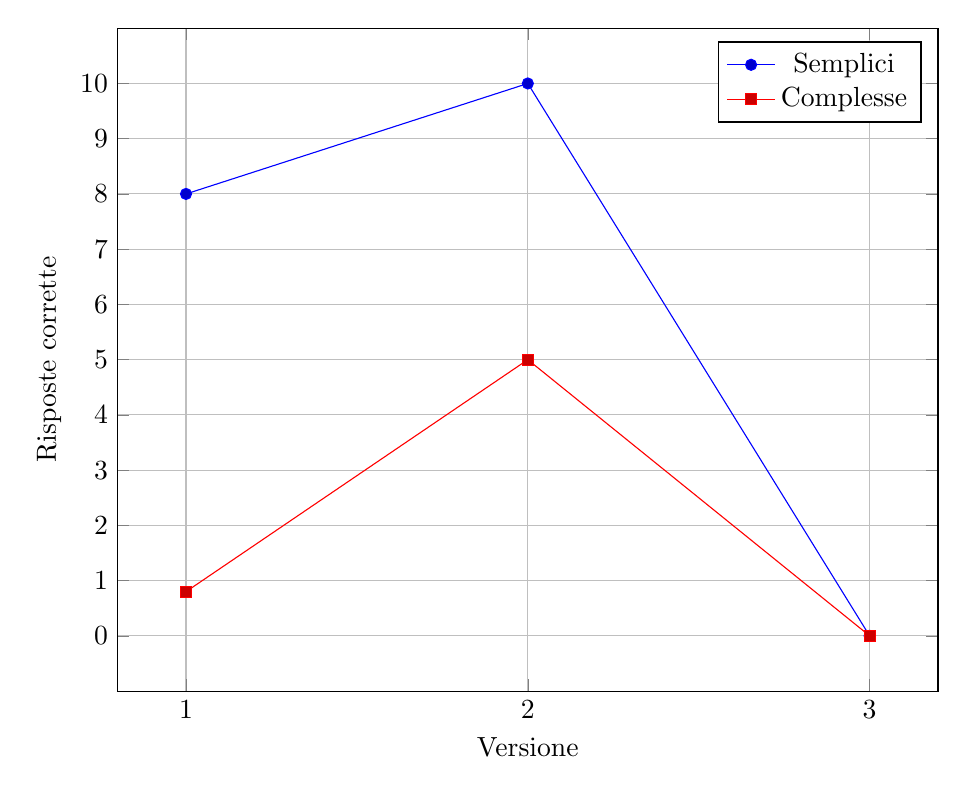
\begin{tikzpicture}
        \centering
        \begin{axis}[
            xlabel={Versione},
            ylabel={Risposte corrette},
            grid=major,
            width=12cm,
            height=10cm,
            xtick={1, 2, 3}, 
            ytick={0, 1, 2, 3, 4, 5, 6, 7, 8, 9, 10}
        ]
        \addplot coordinates {
            (1, 8)
            (2, 10)
            (3, 0)
        };
        \addlegendentry{Semplici}

        \addplot coordinates {
            (1, 0.8)
            (2, 5)
            (3, 0)
        };
        \addlegendentry{Complesse}
        
        \end{axis}
    \end{tikzpicture}
    \caption{Grafico risposte corrette su versione - HTML}

\end{figure}
    
\begin{figure}[H]
    
    \centering
    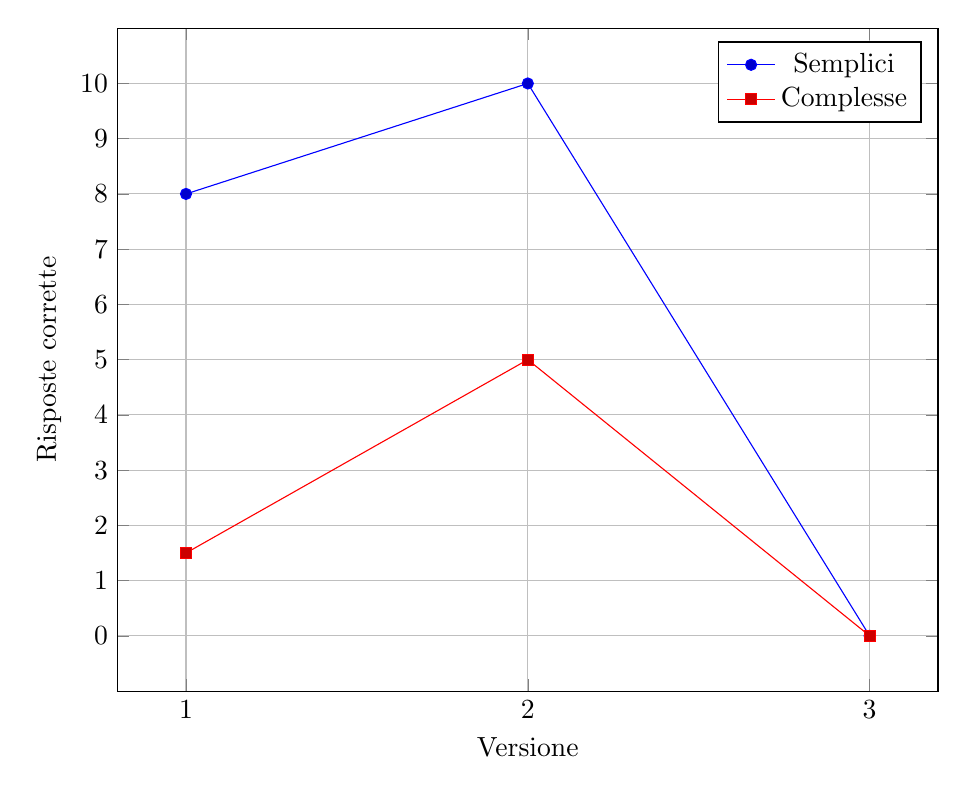
\begin{tikzpicture}
        \centering
        \begin{axis}[
            xlabel={Versione},
            ylabel={Risposte corrette},
            grid=major,
            width=12cm,
            height=10cm,
            xtick={1, 2, 3}, 
            ytick={0, 1, 2, 3, 4, 5, 6, 7, 8, 9, 10}
        ]
        \addplot coordinates {
            (1, 8)
            (2, 10)
            (3, 0)
        };
        \addlegendentry{Semplici}

        \addplot coordinates {
            (1, 1.5)
            (2, 5)
            (3, 0)
        };
        \addlegendentry{Complesse}
        
        \end{axis}
    \end{tikzpicture}
    \caption{Grafico risposte corrette su versione - Docx}

\end{figure}



